\chapter{MINERAÇÃO DE DADOS}

A mineração de dados é uma área da ciência da computação que permite inferir conhecimento a partir de uma massa de dados específica de um fenômeno ou evento qualquer.


Em particular, a mineração de dados contempla a inferência de modelos direcionados por dados, ou seja, modelos derivados unicamente a partir de conjuntos de dados de entrada e de saída específicos de um dado fenômeno ou evento. Utilizam tipicamente um enfoque denominado aprendizado de máquina (machine learning), que basicamente é uma forma de estatística aplicada com enfase no uso de computadores para estimar funções, em geral, complicadas em um conjunto de dados.

A mineração de dados é frequentemente confundida com o processo mais amplo de descoberta de conhecimento em base de dados (KDD- Knowledge Discovery in Databases), a qual é definida como a extração de padrões e desenvolvimento de representações associados ao conhecimento de um processo ou fenômeno a partir de um conjunto de dados associados. A mineração de dados é apenas uma etapa deste processo, sendo definida como a extração de padrões em um conjunto de dados. As diferenças ficam mais claras as sumarizando as etapas contidas em um processo de KDD:

\begin{enumerate}
\item {\bf Limpeza de dados}: remoção de dados com ruído, inconsistentes e incompletos;
\item {\bf Integração de dados}: combinação de múltiplas fontes de dados, por meio de operações como união e intersecção de tabelas;
\item {\bf Seleção de dados}: os dados considerados relevantes ao processo são extraídos do banco de dados;
\item {\bf Transformação de dados}: os dados são transformados e consolidados em uma forma mais apropriada para mineração, sendo por exemplo discretizados, normalizados, agrupados;
\item {\bf Mineração de dados}: é a etapa do KDD associada com a aplicação de algoritmos estatísticos, de reconhecimento de padrões ou de inteligência computacional, como por exemplo, redes neurais, árvores de decisão, visando a extração de padrões, juntamente com a avaliação dos modelos desenvolvidos, por exemplo, medir o desempenho de um sistema de classificação;
\item {\bf Apresentação do conhecimento}: técnicas de visualização e representação dos dados são usadas para exibir o conhecimento extraído aos usuários.
\end{enumerate} 

O processo de KDD é iterativo, como pode ser visto na Figura \ref{fig:kdd} no sentido em que etapas podem ser revistas e reexecutadas em função dos resultados obtidos.

\begin{figure}[H]
\centering
\tikzstyle{block} = [rectangle, minimum width=3cm, minimum height=1cm,text centered, draw=black]
\tikzstyle{arrow} = [thick,->,>=stealth]
\tikzstyle{edges} = [->, bend left]
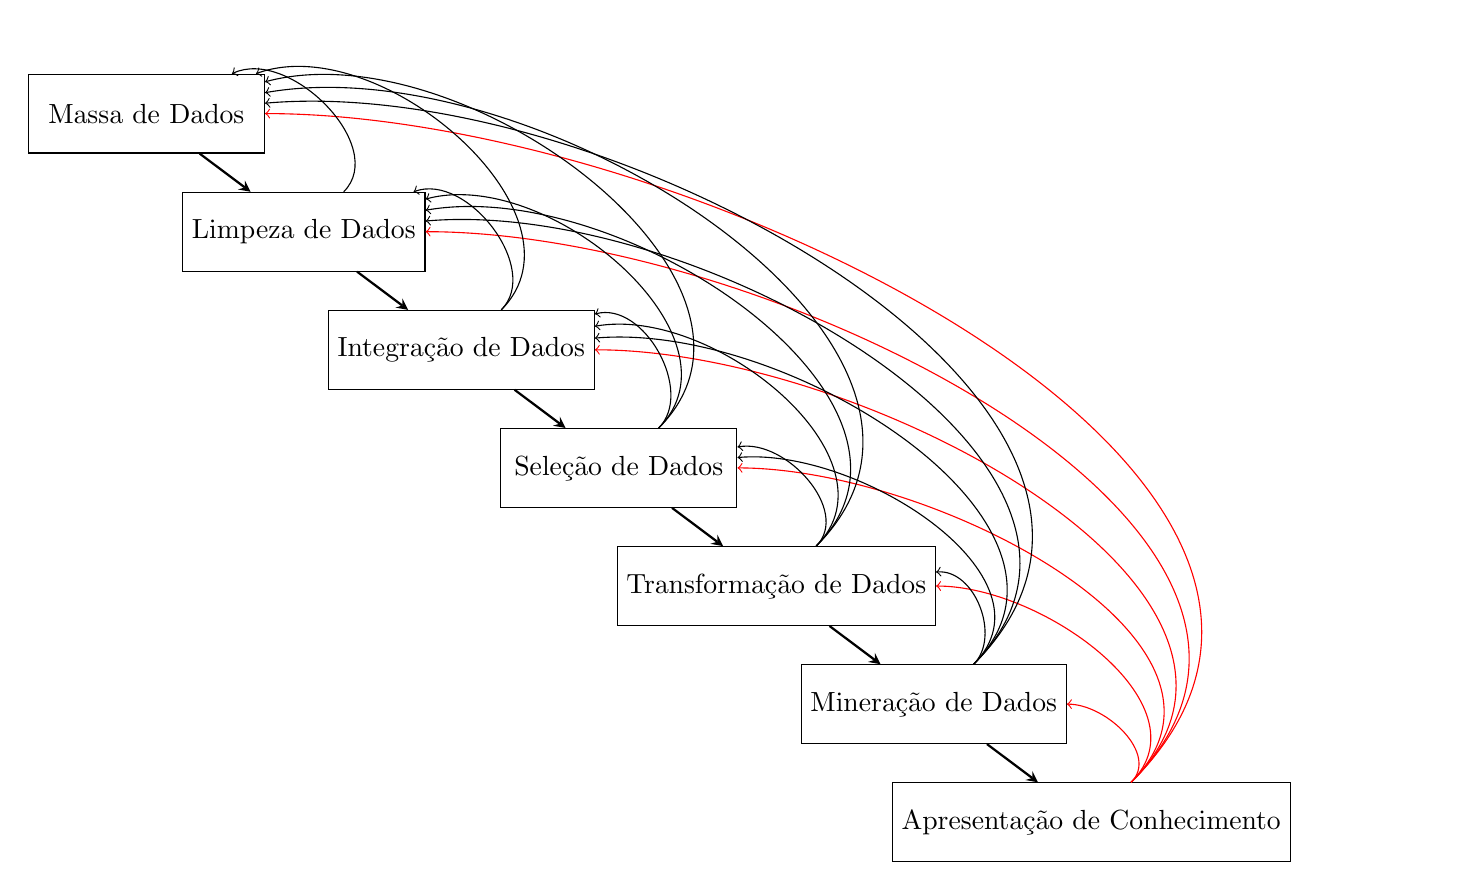
\begin{tikzpicture}[node distance=2cm]
\node (mdados) [block] at (0,0) {Massa de Dados};
\node (ldados) [block] at (2, -1.5) {Limpeza de Dados};
\node (idados) [block] at (4, -3) {Integração de Dados};
\node (sdados) [block] at (6, -4.5) {Seleção de Dados};
\node (tdados) [block] at (8, -6) {Transformação de Dados};
\node (midados) [block] at (10, -7.5) {Mineração de Dados};
\node (aconh)  [block] at (12, -9){Apresentação de Conhecimento};

\draw [arrow] (mdados) -- (ldados);
\draw [arrow] (ldados) -- (idados);
\draw [arrow] (idados) -- (sdados);
\draw [arrow] (sdados) -- (tdados);
\draw [arrow] (tdados) -- (midados);
\draw [arrow] (midados) -- (aconh);

\draw [->, red] (aconh) to [out=45,in=0] (midados);
\draw [->, red] (aconh) to [out=45,in=0] (tdados);
\draw [->, red] (aconh) to [out=45,in=0] (sdados);
\draw [->, red] (aconh) to [out=45,in=0] (idados);
\draw [->, red] (aconh) to [out=45,in=0] (ldados);
\draw [->, red] (aconh) to [out=45,in=0] (mdados);

\draw [->] (midados) to [out=45,in=5] (tdados);
\draw [->] (midados) to [out=45,in=5] (sdados);
\draw [->] (midados) to [out=45,in=5] (idados);
\draw [->] (midados) to [out=45,in=5] (ldados);
\draw [->] (midados) to [out=45,in=5] (mdados);

\draw [->] (tdados) to [out=45,in=10] (sdados);
\draw [->] (tdados) to [out=45,in=10] (idados);
\draw [->] (tdados) to [out=45,in=10] (ldados);
\draw [->] (tdados) to [out=45,in=10] (mdados);

\draw [->] (sdados) to [out=45,in=15] (idados);
\draw [->] (sdados) to [out=45,in=15] (ldados);
\draw [->] (sdados) to [out=45,in=15] (mdados);

\draw [->] (idados) to [out=45,in=20] (ldados);
\draw [->] (idados) to [out=45,in=20] (mdados);

\draw [->] (ldados) to [out=45,in=25] (mdados);
\end{tikzpicture}
\caption{Passos de um processo de KDD. Fonte: Próprio Autor.}
\label{fig:kdd}
\end{figure}

\section{Aprendizagem de máquina}

A aprendizagem de máquina faz uso de algoritmos que são capazes de aprender a partir dos dados, que são ainda agrupados pelo termo {\bf algoritmo de aprendizado de máquina}. Note que esta definição é incompleta, uma vez que não se definiu o que significa aprender a partir dos dados. Assim, considere uma tupla $(P, D, M)$ onde $T$ corresponde à tarefa, $D$ ao conjunto de dados (domínio) e $M$ a métrica, diz-se que um algoritmo aprende com relação ao problema $P$, ao conjunto de dados $D$ e a métrica $M$, se a sua performance no tratamento do problema $P$, avaliado segundo a métrica $M$ melhora conforme itera sobre os dados. 

Basicamente, pode ser visto como o processo de estimar (ajustar) uma função segundo algum objetivo (métrica) a um conjunto de dados. Também é adequado definir o termo função, portanto, sejam $X$ e $Y$ dois conjuntos não vazios, que podem ou não ser iguais, e uma regra, ou conjunto de regras, $f$ que assina cada elemento $x$ de $X$ a um único elemento $y$ em $Y$, um {\bf função} consiste de uma tupla formada por $(X, Y, f)$. Assim, termos como modelo, estimador, preditor são sinônimos do termo função, pois são entendidos como uma realização do algoritmo de aprendizagem para um conjunto de dados, ou seja, um conjunto de regras inferidas dos dados pelo algoritmo.

Um problema $P$ pode ser descrito pela maneira trata um amostra $({\bf x}, y)$ ou $({\bf x})$ do domínio $D$, isto é, o que ela faz ou como processa uma instância. Esta, por sua vez, corresponde a um conjunto de características, atributos ou variáveis que foram quantificadas de algum objeto ou evento que se deseja estudar. Quando uma amostra é da forma $({\bf x}, y)$, diz-se que a instância apresenta um rótulo ou resposta indicado por $y$, enquanto amostras da forma $({\bf x})$ são ditas não rotuladas. O termo ${\bf x}$ também pode ser denominado de atributos de informação, variáveis preditoras, entres outras, enquanto o termo $y$ como como atributo de decisão. Os dados também podem ser numéricos, quantitativos, ou qualitativos. Estes últimos são dados categóricos, que correspondem à atribuição de rótulos que os qualificam.

Uma definição formal de um problema seria um tanto trabalhosa e foge do escopo deste trabalho, entretanto, é possível iniciar a construção uma imagem mental deste por meio de exemplos:

\begin{itemize}
\item Um problema de classificação: neste tipo de problema o objetivo é determinar uma função $f$ que mapeia cada amostra $\bf x$ a uma categoria $j$, em um conjunto de $n$ categorias $\{0,..,n-1\}$;
\item Um problema de regressão: neste tipo de problema o objetivo é determinar uma função $f$ que dado uma instância $\bf x$ prediga um valor numérico.
\end{itemize}

Um segundo aspecto com relação ao problema se refere a maneira pela qual os dados são tratados pelo algoritmos. Neste contexto, os algoritmos de aprendizado de máquina são agrupados basicamente em dois grandes grupos: os supervisionados e os não-supervisionados. Na última década apareceram variações, tais como, algoritmos auto-supervisionados, ou semi-supervisionados, que não são abordados aqui. No caso dos supervisionados, um algoritmo é ajustado na fase de treinamento a partir de instâncias conhecidas, ou seja, de atributos preditores e os correspondentes atributos respostas. Estes algoritmos são utilizados para tarefas como classificação, predição, regressão. Por outro lado, os algoritmos não-supervisionados buscam inferir conhecimento ao agrupar os dados em conjuntos distintos (sem o conhecimento prévio de seus rótulos) ou ao reduzir a dimensionalidade dos dados, ou ao apresentá-los numa forma distinta ou ao extrair padrões, de forma a permitir uma melhor análise do fenômeno ou evento de estudo.

O grande desafio das técnicas de aprendizagem de máquina é que estas precisam apresentar bom desempenho em amostras de dados diferentes das usadas no treinamento. Assim, define-se o conceito de generalização que é a capacidade de apresentar um bom desempenho em amostras de dados não observadas previamente. Usualmente, antes da fase de treinamento de um algoritmo de aprendizagem de máquina, o domínio $D$ é particionado em dois subconjuntos, um de treinamento e um de validação. O subconjunto de treinamento é utilizado na fase de ajuste do modelo, isto é, o treinamento, e a ele por meio de uma métrica, pode-se associar um erro de treinamento, que basicamente, mensura quão bens o modelo se ajusta aos dados deste subconjunto. Note que o erro de treinamento pode não fornecer um indicativo de quão bem o modelo se ajusta a dados não observados. Neste ponto, a aprendizagem de máquina começa a ser separar das abordagens usuais de ajuste de funções, pois define o erro de generalização, ou erro de validação, que deve fornecer informações sobre como o modelo se comportar para novas amostras.

O erro de generalização é avaliado mensurando o desempenho do modelo no subconjunto de validação. Em um primeiro analise, não fica claro como é possível a performance no subconjunto de teste apenas observando os dados de treinamento. Assim, neste ponto, faz-se necessário adotar alguns pressupostos a respeito dos dados: as amostras são independentes entre si; o subconjunto de treinamento e o de teste são identicamente distribuídos, e amostrados da mesma distribuição de probabilidade. Logo, pode-se concluir que o valor estimado de ambos os erros devem ser iguais. Todavia, em um problema real de aprendizagem de máquina tais pressupostos não são completamente verdadeiros, e diversas abordagens são adotadas de forma a melhor se aproximar destes. Portanto, em geral, espera-se que o erro esperado de validação seja maior ou igual ao de treino.

Finalmente, determina-se quão bem um algoritmo desempenha seu papel em relação a um conjunto de dados, avaliando sua habilidade de reduzir o erro de treinamento, mantendo a diferença entre o erro de treinamento e o de validação pequenos. Esta habilidade leva a duas dificuldades extremas opostas, o sobreajuste (overfitting) e sobajuste (underfitting). O primeiro ocorre quando a diferença entre os erros de treinamento e validação divergem; o segundo ocorre quando o modelo não é capaz de reduzir suficientemente o erro de treinamento.

A possibilidade de um modelo sofrer de sobreajuste ou sobajuste pode ser quantificada, teoricamente, em termos de sua capacidade, inclusive a tendência de um ou outro pode ser controlada modificando a capacidade do modelo. De uma maneira informal, pode-se dizer que a capacidade está associado ajustar a habilidade do modelo se ajustar a um grande número de funções. Dois pontos práticos podem ser obtidos dessa construção, modelos de baixa capacidade podem não se ajustar de maneira adequada ao subconjunto de treinamento, enquanto modelos com grande capacidade podem se ajustar de maneira excessiva memorizando o conjunto de treinamento, e assim, não generalizando. Estas colocações devem levantar a necessidade de uma escolha adequada de algoritmo e ajuste de seus parâmetros (ver-se-á alguns exemplos posteriormente) frente aos dados a serem tratados.

\section{Métricas}

As métricas podem ser agrupadas segundo a abordagem do problema, isto é, existem métricas que são adequadas para problemas de classificação, existem métricas que são adequadas para problemas de regressão, e analogamente para diversos outros problemas em mineração de dados e aprendizado de máquina.

\subsection{Classificação}

Primeiramente, é necessário definir o conceito de matriz de confusão, uma vez que a partir dela diversas outras métricas são mais facilmente definidas. 

Admita um problema de classificação com $n$ classes, então a matriz de confusão será uma tabela(matriz) onde cada linha representa instâncias em uma classe predita, enquanto cada coluna representa instâncias em uma classe verdadeira, ou inverso. Assim, dado a $i$-ésima linha e a $j$-ésima coluna com $x$ elementos, diz-se que $x$ elementos da $j$-ésima classe foram preditos como da $i$-ésima classe. A Tabela \ref{tab:mc1} ilustra esta configuração, e por exemplo, pode-se dizer que $h$ elementos da Classe 1 foram previstos como sendo da Classe 2, com a segunda coluna pela terceira linha.

\begin{table}[hhh]
\begin{tabular}{l|l|c|c|c|c}
\multicolumn{2}{c}{}&\multicolumn{3}{c}{Verdadeiro}&\\ \cline{3-5}
\multicolumn{2}{c|}{}&Classe 0& Classe 1 & Classe 2&\multicolumn{1}{c}{Total}\\ \cline{2-5}
\multirow{3}{*}{Predito}& Classe 0 & $a$ & $b$ & $c$ & $a+b+c$\\ \cline{2-5}
                        & Classe 1 & $d$ & $e$ & $f$ & $d+e+f$\\ \cline{2-5}
                        & Classe 2 & $g$ & $h$ & $i$ & $g+h+i$\\ \cline{2-5}
\multicolumn{1}{c}{} & \multicolumn{1}{c}{Total} & \multicolumn{1}{c}{$a+d+g$} & \multicolumn{    1}{c}{$b+e+h$} & \multicolumn{1}{c}{$c+f+i$} & \multicolumn{1}{c}{N}\\
\end{tabular}
\caption{Exemplo de matriz de confusão, onde as colunas estão associadas as instâncias verdadeiras e as linhas as instâncias preditas. Fonte: próprio autor.}
\label{tab:mc1}
\end{table}

Enquanto na representação inversa (transposta) diz se que $x$ elementos da $i$-ésima classe foram preditos como da $j$-ésima classe. A Tabela \ref{tab:mc2} apresenta esta configuração, e se pode dizer, por exemplo, que $h$ elementos da Classe 1 foram previstos como sendo da Classe 2, com a segunda linha pela terceira coluna.

\begin{table}[hhh]
\begin{tabular}{l|l|c|c|c|c}
\multicolumn{2}{c}{}&\multicolumn{3}{c}{Predito}&\\ \cline{3-5}
\multicolumn{2}{c|}{}&Classe 0& Classe 1 & Classe 2&\multicolumn{1}{c}{Total}\\ \cline{2-5}
\multirow{3}{*}{Verdadeiro}& Classe 0 & $a$ & $d$ & $g$ & $a+d+g$\\ \cline{2-5}
                           & Classe 1 & $b$ & $e$ & $h$ & $b+e+h$\\ \cline{2-5}
                           & Classe 2 & $c$ & $f$ & $i$ & $c+f+i$\\ \cline{2-5}
\multicolumn{1}{c}{} & \multicolumn{1}{c}{Total} & \multicolumn{1}{c}{$a+b+c$} & \multicolumn{    1}{c}{$d+e+f$} & \multicolumn{1}{c}{$g+h+i$} & \multicolumn{1}{c}{N}\\
\end{tabular}
\caption{Exemplo de matriz de confusão, onde as colunas estão associadas as instâncias preditas e as linhas as instâncias verdadeiras. Fonte: próprio autor.}
\label{tab:mc2}
\end{table}

Uma vez que ambas as representações são equivalentes, isto é, vão fornecer a mesma informação, a escolha por uma ou outra, ficar a cargo do usuário quando responde peguntas como: qual tenho mais afinidade? Qual acho mais simples? Neste, trabalho adotar-se-á a matriz de confusão com o verdadeiro correspondendo as linhas, e o predito as colunas, \ref{tab:mc2}.

Em posse da matriz de confusão, pode-se definir:

\begin{enumerate}
\item {\bf Verdadeiro Positivo (VP):} é o número de elementos que pertencendo à classe $i$ foram corretamente classificados como $i$. Para a Classe 0 é $VP_0=a$. Generalizando, para uma classe $i$ qualquer:
\begin{equation}\label{eq:vp}
VP_i = A_{ii}\mbox{;}
\end{equation}
\item {\bf Falso Positivo (FP):} é o número de elementos que não pertencem à classe $i$, mas que foram classificados como pertencendo à $i$. Para a Classe 0 é $FP_0=b+c$. Generalizando, para uma classe $i$ qualquer:
\begin{equation}\label{eq:fp}
FP_i = \sum_{j=0,j\ne{i}}^{n-1}A_{ji}\mbox{;}
\end{equation}
\item {\bf Verdadeiro Negativo (VN):} é o número de elementos que não pertencem à classe $i$ e foram classificados como não pertencendo à $i$. Para a Classe 0 é $VN_0=e+h+i+f$. Generalizando, para uma classe $i$ qualquer:
\begin{equation}\label{eq:vn}
VN_i = \sum_{j=l=0,j\ne{i}, l\ne{i}}^{n-1}A_{jl}\mbox{;}
\end{equation}
\item {\bf Falso Negativo (FN):} é o número de elementos que pertencendo à classe $i$, foram erroneamente classificados como não pertencendo à $i$. Para a Classe 1 é $FN_0=d+g$. Generalizando, para uma classe $i$ qualquer:
\begin{equation}\label{eq:fn}
FN_i = \sum_{j=0,j\ne{i}}^{n-1}A_{ij}\mbox{;}~
\end{equation}
\end{enumerate}

onde na expressões \eqref{eq:vp}-\eqref{eq:fn}, $A$ é a matriz de confusão, $n$ é o número de classes, $i,j,l\in{0,...,n-1}$, e os exemplos são dados com relação a Tabela \ref{tab:mc2}.

Utilizando as definições de Verdadeiro Positivo e suas correlatas é possível estabelecer um enorme conjunto de métricas, como por exemplo, acurácia, precisão, especificidade entre outras. Neste texto, apresentar-se-á a definição das duas primeiras, assim como o porquê da adoção de uma em relação a outra.

A {\bf acurárcia} (acc) é uma das métricas mais tradicionais para o tratamento de problemas de classificação. E é definida como o número total de predições corretas sobre o número total de elementos. Seja $A$ uma matriz de confusão associada a um problema com $n$ classes, então a acurácia é dada por:

\begin{equation}
acc=\frac{\sum_{i=0}^{n-1}A_{ii}}{\sum_{i=0,j=0}^{n-1}A_{ij}}\mbox{.}
\end{equation}

Agora, considere um problema com 3 classes, e que o número de elementos da Classe 1 e 2 combinados seja $x$. Admita ainda que o classificador acerte todos as instâncias da Classe 0, porém erre todas as demais duas classes, e que a Classe 0 sozinha tenha $x$ elementos, então a acurácia será $1/2$ ou 0,5. Considere agora que a Classe 0 tenha $2x$ instâncias, neste caso a acurácia será $2/3$ ou 0,6. Um aumento no número de elementos da Classe 0 leva um aumento da acurácia, entretanto as Classes 1 e 2 são erroneamente classificadas, portanto neste caso, a acurácia não é capaz de avaliar o classificador. 

Conjuntos de dados onde o número de elementos por classes são diferentes por ordens de grandezas, como o exemplo estabelecido no parágrafo anterior. são ditos não balanceados e acurácia como definida é incapaz de avaliar classificadores desenvolvido em cima destes dados. Portanto, é necessário definir uma nova métrica, neste caso a precisão, assim seja $A$ a matriz de confusão já apresentada anteriormente, a precisão por classe é dada por:

\begin{equation}
precision_i=\frac{VP_i}{VP_i+FP_i}\mbox{.}
\end{equation}

A precisão para uma dada classe por ser entendida como a proporção de resultados verdadeiros que são definitivamente verdadeiros. E a precisão fica dada por uma média aritmética sobre a precisão de cada classe. Esta é a métrica adotada nos problemas de classificação discutidos nesta proposta.

\subsection{Regressão}

O {\bf erro quadrático médio} (mse) é definido por 

\begin{equation}\label{eq:mse}
mse=\frac{1}{n}\sum_{i=1}^n(y_i-\hat{y}_i)^2\mbox{,}~
\end{equation}

onde $n$ é o número de instâncias a serem preditas (avaliadas), $y_i$ a variável alvo para amostra $i$ e $\hat{y}_i$ o valor predito para a amostra $i$. Esta medida é uma das mais aplicadas, não somente no contexto, de problemas de regressão, mas também nos problemas de otimização em aprendizagem de máquina que necessitem de funções diferenciáveis. Por ser definida em termos de uma operação de média, existem distribuições dos dados a serem preditos para os quais essa métrica é incapaz de avaliar de maneira satisfatória o desempenho do regressor (distribuições altamente localizadas) em uma analogia com o problema de classificação com classes não balanceadas. 

%Este fato pode ser melhor visualizado por um processo de discretização da regressão, o que basicamente é a associação de um histograma a distribuição alvo tal que cada elemento do histograma fique associado a uma classe diferente. 

Deste modo faz necessário avaliar uma métrica que seja capaz de mensurar de maneira mais adequada erros em regiões menos localizadas da distribuição, para tal adotou-se o {\bf erro absoluto máximo} (mae) definido por:

\begin{equation}
mae=\mbox{max}|y_{i}-\hat{y}_i|\mbox{,}~
\end{equation}

onde $i$ vária entre 1 e $n$, com este sendo o úmero de instâncias a serem preditas e $y_i$ e $\hat{y}_i$ sendo respectivamente a variável alvo e o valor predito para a amostra $i$.

\section{Algoritmo: Árvores}

Métodos baseados em árvores particionam os espaço de atributos preditores em um conjunto de retângulos, e então aproxima cada um destes por uma simples função, por exemplo, uma constante. Existem diferentes algoritmos baseados em árvores, CART, C4.5, C4, neste texto discutir-se-á a CART. A Figura \ref{fig:tree} apresenta uma representação visual de uma estrutura de árvore ajustada para um dos conjunto de dados discutido no Capítulo \ref{ch:revisonrezende}.

\begin{figure}[H]
\centering
\makebox[\textwidth][c]{\includegraphics[width=1.3\linewidth]{Figuras/tree.png}}
\caption{Fonte: Próprio Autor.}
\label{fig:tree}
\end{figure}


Considere um problema de regressão com duas variáveis preditoras $x_1$ e $x_2$ e uma resposta contínua $y$, cada um destes tomando valores entre $[0,1]$. Cada partição do espaço de atributos modela $y$ por uma constante diferente. Se as linhas de partições forem definidas definidas de maneira arbitrária, apesar de apresentarem simples descrições, tal como $x_2=c$, a região resultante pode apresentar uma descrição de difícil tratamento. Assim, é interessante restringir a maneira pela o qual as partições são criadas. A limitação mais natural a ser adotada é que as partições sejam definidas recursivamente dividindo o espaço em duas sub-regiões (recursão binária), em outras palavras, inicialmente o espaço de atributos é divido em duas regiões, neste caso, adota-se modelar a resposta $y$ pelo valor médio em cada região. Então, uma destas regiões ou ambas são divididas em mais duas regiões. Tal procedimento é aplicado até que alguma condição de parada seja alcançada. 

A divisão do espaço é realizada segundo algum critério, tal que se deseja obter o melhor ajuste. Finalmente, o correspondente modelo de regressão para a variável $y$ fica definido por:

\begin{equation}\label{eq:treeresponse}
\hat{f}(x)=\sum_{m=1}^Mc_mI(x\in{R_m})\mbox{,}~
\end{equation}

onde $R_m$ indica a $m$-ésima região, $x$ é um elemento do espaço de atributos, $c_m$ é a constante que aproxima $y$ na $m$-ésima região, $M$ é o número de regiões, e $I$ é uma função identidade definida por

\begin{equation}
I(x\in{R_m})=\Big\{\begin{array}{cc}
0,&\mbox{se}\, x\notin{R_m}\mbox{,}\\ 
1,&\mbox{se}\, x\in{R_m}\mbox{.}
\end{array}
\end{equation}

\noindent
para este exemplo, $M=2$ e $x$ é da forma $(x_1, x_2)$. Um importante ganho advindo da restrição em recursão binária, é que a representação da árvore passa a ter uma simples interpretação, onde uma simples condição em cada nó, define os subnós. 

O processo de construção de uma árvore depende se o problema a ser tratado é de regressão ou classificação, o que será discutido nas próximas subseções. E alguns dos elementos da estrutura árvore binárias discutidas apresentam nomes, e condições sobre elas que são

\begin{itemize}
\item um nó pode ser de dois tipos, {\bf decisão}, neste caso fica associado um subconjunto, e uma regra, que particiona esta em duas novas sub-regiões, ou {\bf folha};
\item um nó somente pode dividir uma região em duas sub-regiões ou em nenhuma, no primeiro caso diz-se que ele é um pai, que gera dois filhos, e cada filho está associado a um ramo, no segundo caso ele é uma folha;
\item folha é um nó associado ao final da árvore, portanto o conjunto associado a ele não pode ser dividido, em outras palavras, ele não pode ter filhos, e assim, a cada folha fica associado uma partição e uma constante;
\end{itemize}


\subsection{Árvores de Regressão}

Admita que o conjunto de dados apresente $p$ atributos preditores e um atributo resposta, e um total de $N$ instâncias, ou seja, é da forma $(\bf{x}_i,y_i)|i\in\{1,...,N\}$, com $\bf{x}_i=(x_{i,1}, x_{i,2}, ..., x_{i,p})$. O papel do algoritmo é operar sobre este conjunto de dados e automaticamente decidir em qual variável dividir, qual o ponto (valor) para dividir, e a forma que a árvore deverá assumir. Considere inicialmente que o espaço esteja particionado em $M$ regiões $R_1,...,R_M$, e que a reposta seja ajustada por uma constante $c_m$ em cada região, \eqref{eq:treeresponse}. Ir-se-á adotar como critério para a divisão minimização do erro quadrático médio \eqref{eq:mse}, isto é, o mse em cada sub-região, traduzido na expressão

\begin{equation}\label{eq:a}
\min\frac{1}{N}\sum_{i=1}^N(y_i-\hat{f}(x_i))^2\mbox{.}~
\end{equation}

Avaliando a expressão \eqref{eq:a} com relação aos parâmetros $c_m$, isto é, derivando a expressão com relação a $c_m$ e igualando a zero, obtém-se

\begin{align}
\sum_{i=1}^N(y_i-f(x_i))frac{\partial(f(x_i))}{\partial{c_l}}=&\,0 \nonumber \\
\sum_{i=1}^N(y_i-\sum_{m=1}^Mc_mI(x\in{R_m}))I(x\in{R_l})=\,&0 \nonumber \\
\sum_{i=1}^N(y_i)I(x\in{R_l}) - \sum_{i=1}^N\sum_{m=1}^Mc_mI(x\in{R_m})I(x\in{R_l})=\,&0 \nonumber\\
\sum_{i=1}^N(y_i)I(x\in{R_l}) - c_l \#R_l=\,&0\mbox{,}~
\end{align}

ou

\begin{equation}\label{eq:b}
\hat{c}_l=\frac{1}{\#R_l}\sum_{i|x_i \in{R_l}}y_i\mbox{,}
\end{equation}

onde $\#R_l$ indica a cardinalidade da partição $R_l$, isto é, o número de elementos da região $R_l$, finalmente o lado direito da expressão \eqref{eq:b} corresponde a média sobre os valores de $y_i$ que estão na região $R_l$. Adotar-se-á a seguinte notação para simplificar a expressão \eqref{eq:b} $\hat{c}_m=\mu(y_i|x_i\in{R_l})$. 

Encontrar a melhor partição que minimiza o mse de maneira geral como definido acima é um problema quase intratável computacional, entretanto, é possível adotar-se uma abordagem gulosa, que lida com um problema semelhante. Comece com o conjunto de todos os dados, considere dividir este utilizando a variável $j$ das $p$ variáveis, em um ponto $s$ dos $N$ pontos, definindo-se assim duas regiões

\begin{align}
R_1(j,s) = \{x\,|\,x_j\le{s}\}\\
R_2(j,s) = \{x\,|\,x_j>s\}\mbox{.}
\end{align}

Então, procura-se a variável $j$ e ponto $s$ que resolvem o problema de minimização

\begin{equation}
\min_{j,s}\left[\min_{c_1}\sum_{x_i\in{R_1(j,s)}}(y_i-c_1)^2+\sum_{x_i\in{R_2(j,s)}}(y_i-c_2)^2\right]\mbox{.}
\end{equation}

Note entretanto que já foi resolvido um problema similar para a minimização da parte interna $(y_i-c_1)$ para qualquer que seja $j$ e $s$:

\begin{equation}
\hat{c}_1=\mu(y_i|x_i\in{R_1(j,s)})\quad\mbox{e}\quad\hat{c}_2=\mu(y_i|x_i\in{R_2(j,s)})\mbox{.}
\end{equation}

Assim, para cada variável de divisão $j$, a determinação do ponto de divisão $s$ pode ser realizada rapidamente, varrendo todos os possíveis valores, por exemplo, tal que encontra o melhor par $(j,s)$ para cada região seja tratável. Uma vez encontrado este par, particionasse a região em duas sub-regiões, e aplica-se o processo para cada uma das duas sub-regiões. Este processo é repetido para cada nova sub-região até que algum critério de parada seja alcançado.

O tamanho da árvore governa a complexidade do modelo, e um valor ótimo deve ser escolhido segundo os dados. Assim, existem diferentes critérios para dividir ou não um nó, por exemplo, divida o nó somente se o decréscimo no mse foi maior que um determinado valor.


\subsection{Árvores de Decisão}

No caso da variável resposta estar associada a um problema de classificação, as modificações no algoritmo se resumem a modificação do critério de divisão do nó e os critérios de parada. Defini-se a medida de impureza de um nó $m$ com relação a uma árvore $T$, para um problema de regressão, por

\begin{equation}
Q_m(T)=\frac{1}{\#R_m}\sum_{x_i\in{R_m}}(y_i-\hat{c}_m)^2\mbox{,}~
\end{equation}

note que quanto mais $Q_m(T)$ tende a $0$, mais se diz que o nó é puro. Observando também a relação de impureza fica claro que ela apresenta relação fundamental com o critério de divisão de um nó, entretanto para um problema de classificação, tal relação não é adequada. Assim, é necessário definir ao menos uma medida para este tipo de problema. Seja $m$ um nó de um árvore em um problema de classificação, representando uma região $m$ com $N_m$ instâncias ($N_m=\#R_m$), define-se

\begin{equation}
\hat{p}_{mk}=\frac{1}{N_m}\sum_{x_i\in{R_m}I(y_i=k)}\mbox{,}~
\end{equation}

a proporção de elementos da $k$-ésima classe no nó $m$. A classe associada ao nó $m$ denotada por $k(m)$ é $k(m)=\max_k\hat{p}_{mk}$, ou seja, a classe que apresenta o maior número de elementos neste nó. Assim, pode-se definir algumas medidas de impureza:

\begin{itemize}
\item {\bf Erro de Classificação}
\begin{equation}
\frac{1}{N_m}\sum_{i\in{R_m}}I(y_i\neq{k}(m))=1-\hat{p}_{mk(m)}\mbox{;}
\end{equation}
\item {\bf Indice Gini}
\begin{equation}
\sum_{k\neq{k}'}\hat{p}_{mk}\hat{p}_{mk'}=\sum_{k=1}^{K}\hat{p}_{mk}(1-\hat{p}_{mk})\mbox{;}
\end{equation}
\item {\bf Entropia Cruzada}
\begin{equation}
-\sum_{k=1}^K\hat{p}_{mk}\log\hat{p}_{mk}\mbox{.}
\end{equation}
\end{itemize}

Finalmente, o critério de divisão fica definido como maximizar o nível de pureza ao dividir um nó. Considere um nó $m$ com $N_m$ elementos, tal que cada elemento tenha $p$ variáveis preditoras e um variável resposta que indica a classe da amostra. Assim, de maneira gulosa, busca-se uma variável $j$ e um ponto de divisão $s$ tal que a soma da medida de impureza de cada sub-região $Q_{x_j\le{s}}(T)$ e $Q_{x_j>{s}}(T)$ seja mínima, ou

\begin{equation}
\min_{j,s}\left[Q_{x_j\le{s}}(T)+Q_{x_j>{s}}(T)\right]\mbox{.}
\end{equation}

A escolha da medida de impureza depende do algoritmo, a CART utiliza o índice Gini.

\section{Técnicas de Conjunto}

A grande maioria dos algoritmos de aprendizagem de máquina, usualmente, ajustam um único modelo para resolver um problema, em contraste, existe uma classe de métodos que adotam a abordagem de construir um conjunto de modelos e combiná-los de forma a tratar o problema. Essa classe é denominada de métodos de conjunto do inglês ``ensemble methods'' ou métodos baseados em comitê.

Um conjunto contém um número de modelos de base, os quais são gerados a partir dos dados de treinamento por um algoritmo de aprendizagem de base. A maioria das técnicas de conjunto utilizam um único algoritmo de aprendizagem de base, e neste caso são denominados de conjuntos homogêneos. Todavia em princípio não existe nenhuma restrição para a utilização de diferentes algoritmos, neste caso, tem-se conjuntos heterogêneos.

A capacidade de generalização de um conjunto é maior do que os modelos de base. Em geral, utiliza-se algoritmos de base denominados de aprendizes fracos que são aqueles cuja previsão é um pouco melhor do que um sorteio aleatório. Assim, o papel da técnica de conjuntos é melhor os aprendizes fracos, onde suas combinações o tornam um aprendiz forte, isto é, aquele que gera modelos capazes de predições bem acuradas. O cerne da técnica pode ser traduzido no ditado popular ``a união faz a força''.

Os métodos de conjunto se tornaram um importante paradigma depois da década de 90, com a publicação de dois trabalhos pioneiros \cite{HANSEN:1990} e \cite{SCHAPIRE:1990}. O primeiro destes mostrou empiricamente que a predição realizada pela combinação de um conjunto de classificadores é em geral mais acurada do que a feita por um único bom classificador. O segundo de caráter teórico mostra que aprendizes fracos podem ser combinados de forma a geral aprendizes fortes. 

Em geral, estes conjuntos são construídos em dois passos, a geração dos modelos de base e, então, a combinação deles. Assim, para a obtenção de um bom conjunto se busca modelos de base tão acurados quanto possível, e tão diversos quanto possível. 

Nas próximas duas subseções ir-se-á discutir dois métodos gerais a respeito de técnicas de conjunto o ``bagging'' e o ``boosting''.

\subsection{Boosting}

O termo ``boosting'' se refere a uma família de algoritmos que são capazes de converter um preditor fraco em um preditor forte. O procedimento geral é bem simples. Considere que um preditor fraco sobre uma distribuição qualquer, e considere um problema de classificação binária como exemplo, ou seja, deseja classificar as amostras em positivo ou negativo. O domínio $D$ é amostrado identicamente e independentemente da distribuição.

Admita agora que o domínio $D$ é divido em 3 regiões $D_1$, $D_2$ e $D_3$, onde cada uma compõem um terço de $D$ e que um preditor fraco tenha um erro de classificação da ordem de 50\%. O objetivo é ter uma acurácia alta, com um erro de classificação próximo de 100\%. Todavia inicialmente, tem-se apenas um preditor fraco $f_1$ que apenas realiza classificações corretas para as regiões $D_1$ e $D_2$ errando todas as classificações para a região $D_3$, neste caso ele tem um erro de classificação de ao menos um terço.

A ideia geral de boosting é corrigir os erros gerados pelo classificador $f_1$, para tal gerasse um novo domínio $D'$ que realce os erros de $f_1$, em outras palavras, foque nas amostras em $D_3$. Então treinasse um novo classificador $f_2$  no domínio $D'$. Este novo classificador apresenta bons resultados para a subregiões $D_1$ e $D_3$, porém apresenta muitos erros para a região $D_2$. Combinando de maneira adequada os classificadores $f_1$ e $f_2$ ter-se-á classificações corretas para $D_1$ e alguns erros para $D_2$ e $D_3$.

Novamente, o mesmo procedimento é adotado, gera-se um novo domínio $D''$ que destaque os erros de classificação cometidos pela combinação de $f_1$ e $f_2$ e treinasse um classificador $f_3$ que produza boas classificações para a região $D_2$ e $D_3$.

Resumidamente, a técnica de ``boosting'' treina um conjunto de preditores sequencialmente e os combinando para gerar um predição, onde cada preditor é treinado focando nos erros dos preditores anteriores.

\subsection{Bagging}

Existem basicamente dois paradigmas centrais nas técnicas de conjuntos. O primeiro é a técnica de conjuntos sequencias (boosting) onde os preditores base são gerados sequencialmente, e o segundo é a técnica de conjuntos paralelo, onde os preditores base são gerados em paralelo (``bagging'') \cite{BREIMAN:1996}.

A principal motivação por trás dos métodos sequencias é explorar a dependência entre os preditores base, uma vez que a performance pode ser melhorada por um processo análogo a redução de resido. Por sua, o cerne dos métodos paralelos é explorar a independência entre os preditores de base, uma vez que o erro pode ser reduzido combinando preditores de base independentes.

Todavia é praticamente impossível obter preditores de base independentes, haja visto que são gerados com base no mesmo conjunto de treinamento. Assim, uma maneira de reduzir a dependência dos preditores se dá pela introdução de aleatoriedade no processo de treinamento, incluindo aqui a própria geração do conjunto de treinamento.

A estratégia de bagging introduz aleatoriedade pela adoção de amostras do subconjunto de treinamento. Os dois elementos principais são a agregação, isto é, a combinação do preditores de base e a amostragem com reposição.

Considere um conjunto de treinamento contendo $m$ amostras $A$, um novo conjunto de $m$ amostras $A_1$ é gerado amostrando com reposição $A$, neste caso, note que alguns exemplos do conjunto $A$ podem aparecer várias vezes, enquanto alguns elementos podem não aparecer. Aplicando este processo $l$ vezes são gerados $l$ conjuntos de amostras com $m$ elementos. Então, cada conjunto é utilizado no treinamento de um modelo de base, quando da aplicação do algoritmo de aprendizagem de base.

A agregação é realizada utilizando procedimentos tradicionais, no caso da regressão se toma a média dos resultados gerados por cada preditor de base, no caso de classificação se toma a classe mais predita pelos preditores de base, em uma analogia com uma votação.

\section{Extreme Gradient Boosting: XGBOOST}

A explicação aqui apresentada sobre o algoritmo XGBOOST é baseada no trabalho de \cite{CHEN:2016}. Considere um conjunto de dados com $N$ amostras e $p$ atributos $\mathcal{D}({\bf x}_i, y_i)$ onde $_{\bf X}\in\mathbb{R}^N$ e $y_i\in\mathbb{R}$, um modelo baseado em um conjunto de árvores utiliza $K$ funções aditivas (árvores) para predizer, estimar, a variável resposta:

\begin{equation}\label{eq:xgboost}
\hat{y}_i=\sum_{k=1}^{K}f_{k}({\bf x}_i)\mbox{,}\,f_{k}\in\mathcal{F}\mbox{,}~
\end{equation}

onde $\mathcal{F}=\{f({\bf x})=c_{q({\bf x})}\}(q:\mathbb{R}^N\to{M},c\in\mathbb{R}^{M})$ é o espaço de árvores de regressão (CART), $q$ representa a estrutura de cada árvore que mapeia uma amostra na correspondente folha, $M$ é o número de folhas na árvore. Cada função $f_k$ corresponde a uma estrutura de árvore completa e independente q e folhas com valor $c$. Assim, para uma dada amostra, utiliza-se as regras de decisões nas árvores dadas por $q$ para classificar em uma folha, e calcular o valor de predição final somando os valores nas correspondentes folhas, dadas por c. A Figura \ref{fig:tree_model}

\begin{figure}[H]
\centering
\makebox[\textwidth][c]{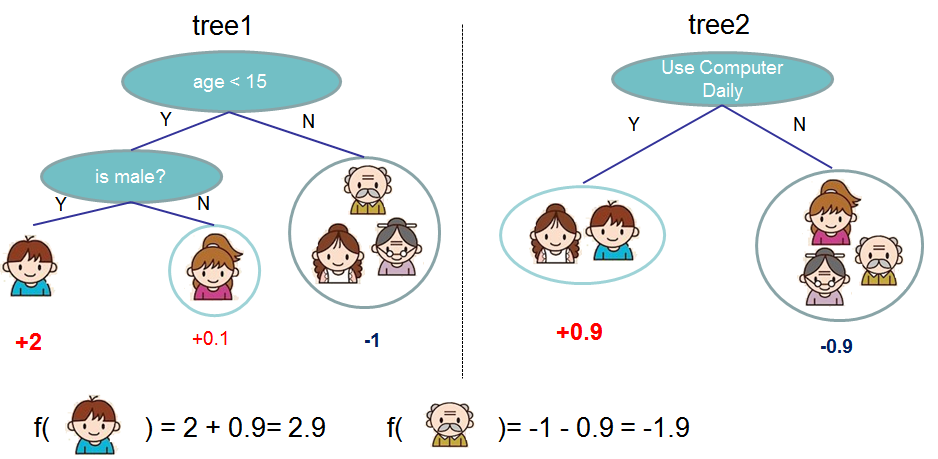
\includegraphics[width=0.8\linewidth]{Figuras/tree_model.png}}
\caption{Modelo de conjunto de árvores. O resultado final para um dada amostra é a soma das predições para cada árvore. Fonte: Adaptado de \cite{CHEN:2016}.}
\label{fig:tree_model}
\end{figure}

O processo de aprendizado deste algoritmo, consiste em determinar as funções $f_k$, para tal, minimiza-se a seguinte função objetivo regularizada:

\begin{equation}\label{eq:xgboostmin}
\mathcal{L}=\sum_{i}l(\hat{y}_i, y_i)+\sum_{k}\Omega{f_k}\mbox{,}~
\end{equation}

\noindent
onde 

\begin{equation}
\Omega(f)=\lambda{T}+\frac{1}{2}\lambda||{\bf c}||^2\mbox{.}
\end{equation}

$l$ é uma função de erro convexa diferenciável que mede a diferença entre o valor predito $\hat{y}_i$ e o valor reposta $y_i$. O segundo termo penaliza a complexidade do modelo. Sua adição suaviza os coeficientes $c$ aprendidos, o que por sua vez reduz a probabilidade de sobreajuste. Note que quando $\gamma=0$, o algoritmo se torna boosting de árvores com gradiente tradicional.

O modelo de conjunto de árvores na equação \eqref{eq:xgboost} inclui funções não analíticas, e o problema de minimização \eqref{eq:xgboostmin} incluí funções com parâmetros e, portanto, não pode ser minimizado tradicionalmente utilizando técnicas de otimização em espaços Euclideanos. Assim, uma abordagem aditiva, análoga ao método guloso adotado na construção de árvores de regressão (CART), é utilizado. Seja, $\hat{y}_{i}^{(t)}$ a predição da $i$-ésima instância na $t$-ésima interação, adiciona-se $f_t$ de forma a minimizar o seguinte objetivo

\begin{equation}
\mathcal{L}^{t}=\sum_{1}^{K}l(y_i, \hat{y}_i^{(t-1)}+f_t({\bf x}_i))+\Omega(f_t)\mbox{.}~
\end{equation}

Utilizando-se de uma aproximação de segunda ordem para o termo $\mathcal{L}^{t}$:

\begin{equation}
\mathcal{L}^{t}\approx\sum_{1}^{K}\left[l(y_i, \hat{y}_i^{(t-1)})+\frac{\partial l(y_i, \hat{y}_i^{(t-1)})}{\partial\hat{y }^{(t-1)}}f_t({\bf x}_i)+\frac{1}{2}\frac{\partial^2 l(y_i, \hat{y}_i^{(t-1)})}{{\partial\hat{y }^{(t-1)}}^2}f_t^2({\bf x}_i)\right]+\Omega(f_t)\mbox{,}~
\end{equation}

cuja a notação pode ser simplificada definindo:

\begin{equation}\label{eq:simpl}
g_i=\frac{\partial l(y_i, \hat{y}_i^{(t-1)})}{\partial\hat{y }^{(t-1)}} \quad \mbox{e} \quad h_i=\frac{\partial^2 l(y_i, \hat{y}_i^{(t-1)})}{{\partial\hat{y }^{(t-1)}}^2}\mbox{,}~
\end{equation}

que são respectivamente os gradientes de primeira e segunda ordem para a função de erro. Descartando termos constantes e utilizando as simplificações definidas em \eqref{eq:simpl}, obtém-se a seguinte função objetivo simplificada no tempo $t$

\begin{equation}\label{eq:nobj}
\mathcal{\tilde{L}}^{t}=\sum_{i=1}^{K}\left[g_if_t({\bf x}_i)+\frac{1}{2}h_if_t^2({\bf x}_i)\right]+\Omega(f_t)\mbox{.}~
\end{equation}

Expandindo a equação \eqref{eq:nobj}, usando que $f_t(x_i)=\sum_{j=1}^{T}c_jI(x_i\in R_j)$ e que $f_t(x_i)^2=\sum_{j=1}^{T}c_j^2I(x_i\in R_j)$:

\begin{align}\label{eq:nobj1}
\mathcal{\tilde{L}}^{t}&=\sum_{i=1}^{K}\left[g_if_t({\bf x}_i)+\frac{1}{2}h_if_t^2({\bf x}_i)\right]+\gamma T + \frac{1}{2}\lambda\sum_{j=1}^Tc_j^2 \\
                       &=\sum_{i=1}^{K}\left[g_i\sum_{j=1}^{T}c_jI(x_i\in R_j)+\frac{1}{2}h_i\sum_{j=1}^{T}c_j^2I(x_i\in R_j)\right]+\lambda{T} + \frac{1}{2}\lambda\sum_{j=1}^Tc_j^2\mbox{,}
\end{align}

trocando $i$ por $j$ e $j$ por $i$ no primeiro termo da expressão \eqref{eq:nobj1} e agrupando-se os termos, tem-se:

\begin{equation}\label{eq:nobj2}
\mathcal{\tilde{L}}^{(t)}=\sum_{j=1}^{T}\left[c_j\sum_{i|{\bf x}_i\in R_j}g_i+\frac{1}{2}c_j^2\left(\sum_{i|{\bf x}_i\in R_j}h_i+\lambda\right)\right]+\gamma{T}\mbox{.}~
\end{equation}

Tomando a variação da equação \eqref{eq:nobj2} com relação a $c_j$, encontra-se que o valor ótimo de  $\hat{c}_j$ para a folha $j$ é dado porquê

\begin{equation}
\hat{c}_j=-\frac{\sum_{i|{\bf x}_i\in R_j}g_i}{\lambda+\sum_{i|{\bf x}_i\in R_j}h_i}\mbox{,}~
\end{equation}

e o correspondente valor ótimo por

\begin{equation}\label{eq:quality}
\mathcal{\tilde{L}}^{(t)}==-\frac{1}{2}\sum_{j=1}^{T}\frac{\sum_{i|{\bf x}_i\in R_j}g_i}{\lambda+\sum_{i|{\bf x}_i\in R_j}h_i}+\gamma T\mbox{.}
\end{equation}

A equação \eqref{eq:quality} pode ser utilizada para medir a qualidade de uma árvore. Seu valor é semelhante a uma medida de impureza, entretanto é derivada de um largo conjunto de funções objetivos. Assim, como aconteceu para a árvore de decisão, é impossível avaliar todas as possíveis árvores, por isso, um algoritmo guloso que inicia com uma única folha (se a árvore tiver apenas um único nó, o original, pela definição de nó folha, ele será uma folha) e adiciona ramos à árvore é utilizado. Considere que $R_E$ e $R_D$ sejam respectivamente o nó da esquerda e da direita após a divisão. Definindo $R=R_E\cup R_D$, a redução de erro (análoga à redução de impureza) após dividir os nós é dador por

\begin{equation}\label{eq:split}
\mathcal{\tilde{L}}_{split}=\frac{1}{2}\left[\frac{\sum_{i|{\bf x}_i\in R_E}g_i}{\lambda+\sum_{i|{\bf x}_i\in R_E}h_i}+\frac{\sum_{i|{\bf x}_i\in R_D}g_i}{\lambda+\sum_{i|{\bf x}_i\in R_D}h_i}-\frac{\sum_{i|{\bf x}_i\in R}g_i}{\lambda+\sum_{i|{\bf x}_i\in R}h_i}\right]-\gamma\mbox{.}
\end{equation}

A fórmula \eqref{eq:split} é usada na prática para avaliar os candidatos de divisão.O algoritmo de busca guloso é apresentado em \ref{al:greedyfind}. A Figura \ref{fig:structscore} apresenta a estrutura do processo de cálculo da divisão.

\begin{algorithm}
\caption{Algoritmo Guloso Exato de Busca de Divisão}\label{al:greedyfind}
\begin{algorithmic}[1]

\State gain $\gets$ 0
\State G $\gets$ $\sum_{i\in R}g_i$
\State H $\gets$ $\sum_{i\in R}h_i$
\For{k=1 to $N$}
    \State G\_L $\gets$ 0
    \State H\_L $\gets$ 0
    \For{j em R ordenado}
        \State G\_L $\gets$ G\_L $+$ $g_j$
        \State H\_L $\gets$ H\_L $+$ $h_j$
        \State G\_R $\gets$ G $-$ $G_L$
        \State H\_R $\gets$ H $-$ $H_L$
        \State value $\gets$ max(value, $\frac{G_L^2}{H_L+\lambda}+\frac{G_R^2}{H_R+\lambda}-\frac{G^2}{H+\lambda}$)
    \EndFor
\EndFor
\end{algorithmic}
\end{algorithm}

\begin{figure}[H]
\centering
\makebox[\textwidth][c]{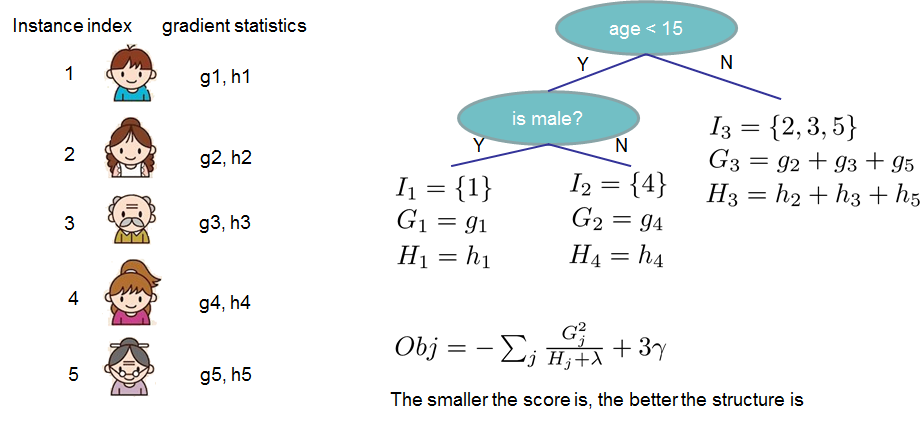
\includegraphics[width=0.8\linewidth]{Figuras/struct_score.png}}
\caption{Estrutura do cálculo de divisão.Apenas é necessário soma o gradiente e o gradiente de segunda ordem da função de erro em cada nó, então aplicar a fórmula \eqref{eq:split} para obter a medida de qualidade. Fonte: Adaptado de \cite{CHEN:2016}.}
\label{fig:structscore}
\end{figure}

O algoritmo combina várias outras técnicas de forma a tratar o problema de sobreajuste e generalizar os resultados, entretanto foge do escopo desta proposta apresentar uma discussão sobre elas. Todavia, algumas destas serão utilizadas neste trabalho, e quando o feito, uma breve introdução a estas será realizada. Finalmente, os principais elementos do algoritmo XGBOOST foram discutidos nesta seção.














